\clearpage
\section{Technische Grundlagen Bluetooth Mesh}\label{sec:TechnischeGrundlagenBluetoothMesh}




\subsection{Netzaufbau und Topologie}\label{sec:NetzaufbauundTopologie}

Nebst dem funktionellen Aspekt übernehmen Nodes unterschiedliche Rollen im Netzaufbau. Ein Node wird als Relay-Node bezeichnet wenn dieser Nachrichten an weitere Teilnehmer weiterleitet. Ein Friend-Node dient als Zugangspunkt für einen Low-Power-Node. Der Low-Power-Node wird dort eingesetzt wo keine konstante Stromversorgung zur Verfügung steht. Dieser geht eine Beziehung mit einem Friend-Node ein. Der Friend-Node speichert alle Nachrichten der LPNs, welche mit ihm eine Beziehung pflegen. In einem festen Zeitintervall fragt der LPN die verpassten Nachrichten beim Friend-Node ab. Dadurch kann der LPN zwischen Abfragen inaktiv bleiben um Energie zu sparen. Um die Interoperabilität zwischen inkompatiblen Bluetooth-Mesh Geräten und einem Mesh-Netzwerk zu ermöglichen existieren Proxy-Nodes. Ein Proxy-Node dient als Schnittstelle in das Netzwerk und erlaubt das Interagieren über Bluetooth-GATT mit dem Mesh. Dies ermöglicht das steuern des Netzwerks über das Smartphone. Die in Abbildung \ref{fig:BTMeshTopology} gezeigt Topologie zeigt die verschiedenen Node-Typen an ihrem Einsatzort. 

\begin{figure} [H]
	\centering
	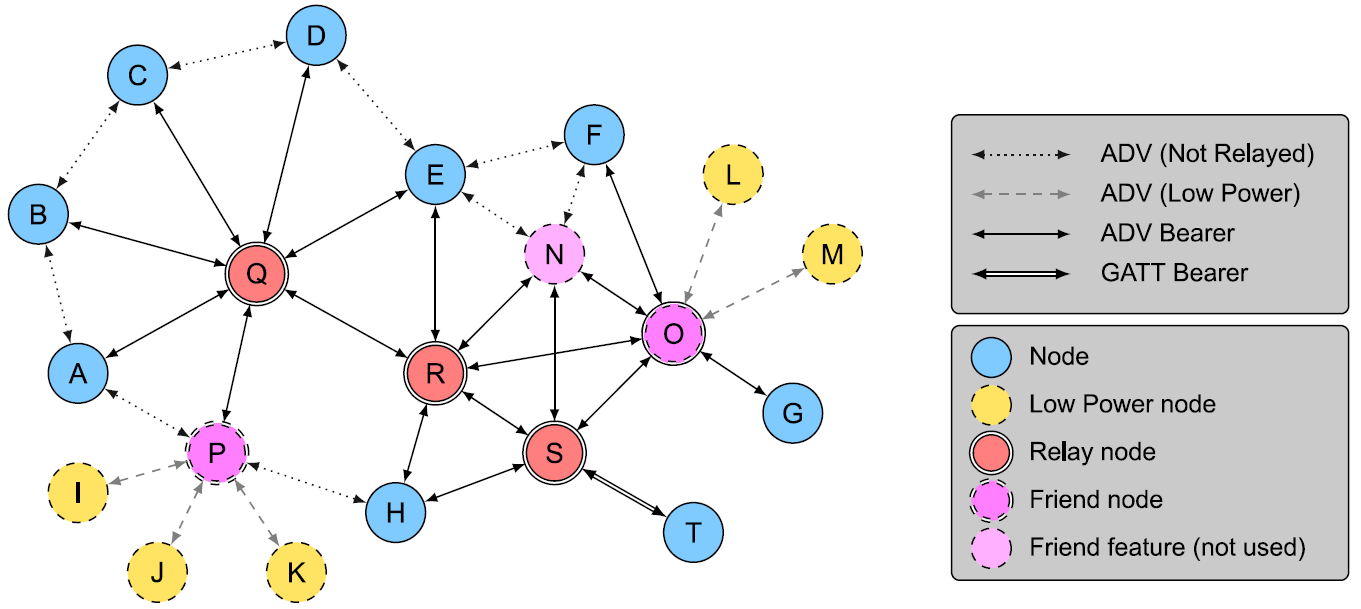
\includegraphics[width=1.0\textwidth]{Bluetooth_Mesh_Topology.PNG}
	\caption{Beispielhafte Topologie eines Bluetooth-Mesh Netzwerks \cite{bluetooth_sig_mesh_netzwerk_spezifikationen_2020}} 
	\label{fig:BTMeshTopology}
\end{figure}


\subsection{Protokoll Stack}\label{sec:BLEMeshProtokollStack}

In diesem Abschnitt wird die Architektur des Mesh-Stacks genauer untersucht. Wie in Kapitel \ref{sec:EinleitungBluetooth} bereits erwähnt basiert der Stack auf Bluetooth Low Energy. Der BLE-Layer dient zur Grundlegenden Schicht des Stacks. Der Zugriff für Mesh-Traffic erfolgt über das GAP-Profil, der für Proxy Traffic über das GATT-Profil. Der Bearer-Layer regelt den Zugriff auf den BLE-Stack. Es existieren verschiedene Bearers. Der GATT-Bearer ermöglicht Geräten ohne GAP Zugriff auf das Netzwerk. Der Advertising-Bearer wird für den Mesh-Traffic benutzt. \\

Der Network-Layer hat folgende Aufgaben zu erfüllen: 

\begin{itemize}
	\item Ver- und Entschlüsselung der Network-PDU
	\item Filtern von nicht relevanten Nachrichten (Adressauflösung)
	\item Relaying von Paketen mittels TTL-Field
\end{itemize}

Zudem bedient dieser Layer verschiedene Bearers und ist dafür verantwortlich das alle relevanten Pakete zur entsprechenden Stelle weitergeleitet werden. \\




\begin{figure} [H]
	\centering
	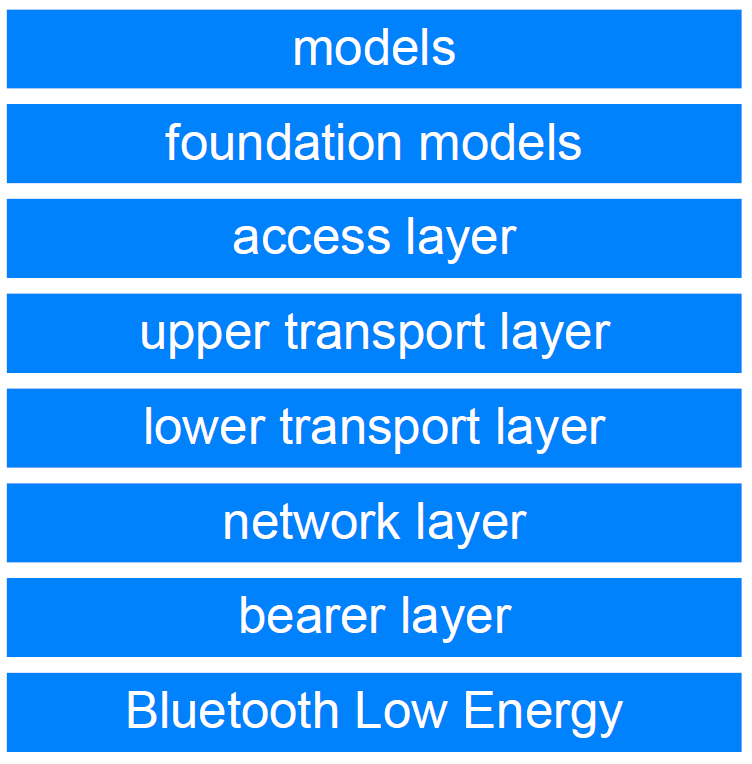
\includegraphics[width=0.5\textwidth]{Bluetooth_Mesh_Stack_Layers.PNG}
	\caption{Bluetooth-Mesh Stack \cite{bluetooth_sig_mesh-technology-overviewpdf_2020}} 
	\label{fig:BTMeshStack}
\end{figure}



\todo[inline]{Erläuterung des Protokoll Stacks. Möglichst viel Grafiken und nur so viel als nötig Prosa.}


\subsection{Grenzen des Stacks}\label{subsec:BLEMeshProtokollStack}

Die Topologie eines Netzwerks beeinträchtigt stark seine Performance. Ist die Node-Dichte sehr hoch, steigt die Wahrscheinlichkeit an das es zu Kollisionen der einzelnen Nachrichten kommt. 

\subsection{Bluetooth Mesh Software Development Kit}\label{sec:ZigbeeSoftwareDevelopmentKit}
\todo[inline]{Eingesetzte SDK und deren Aufbau beschreiben. Allenfalls die wichtigsten API Funktionen genauer erläutern.}


